\documentclass[a4paper,12pt,oneside]{book}
\usepackage[utf8]{inputenc}
\usepackage{sectsty}
\usepackage{graphicx}
\usepackage[table]{xcolor}
\usepackage{array}
\usepackage{algorithm}
\usepackage{algpseudocode}
\usepackage{anysize}
\usepackage{amsmath}
\usepackage{amssymb}
\usepackage[bahasa]{babel}
\usepackage{indentfirst}
\usepackage{geometry}
\usepackage{multirow}
\usepackage{hhline}
\marginsize{4cm}{3cm}{3cm}{3cm}
\usepackage[compact]{titlesec}
\usepackage{etoolbox}
\usepackage{natbib}
\usepackage[bookmarks,hypertexnames=false,debug]{hyperref}
\usepackage{bookmark}
\usepackage{float}
\usepackage{tabularx}
\usepackage{booktabs}

\makeatletter
\patchcmd{\ttlh@hang}{\parindent\z@}{\parindent\z@\leavevmode}{}{}
\patchcmd{\ttlh@hang}{\noindent}{}{}{}
\makeatother

\chapterfont{\centering}
\newcommand{\bigsize}{\fontsize{16pt}{14pt}\selectfont}
\chapterfont{\centering\bigsize\bfseries}
\sectionfont{\large\bfseries}
\usepackage{tikz}
\usetikzlibrary{shapes.geometric, arrows, positioning}
\renewcommand{\thechapter}{\Roman{chapter}}
\renewcommand\thesection{\arabic{chapter}.\arabic{section}}
\renewcommand\thesubsection{\thesection.\arabic{subsection}}
\renewcommand\theequation{\arabic{chapter}.\arabic{equation}}
\renewcommand\thefigure{\arabic{chapter}.\arabic{figure}}
\renewcommand\thetable{\arabic{chapter}.\arabic{table}}

\renewcommand\bibname{Daftar Pustaka}
\addto{\captionsbahasa}{\renewcommand{\bibname}{Daftar Pustaka}}
\usepackage{fancyhdr}
\pagestyle{fancy}
\lhead{}
\chead{}
\rhead{}
\lfoot{}
\fancyfoot[C]{\raisebox{0.5cm}{\thepage}}
\fancypagestyle{plain}{\fancyhf{}\fancyfoot[C]{\raisebox{0.5cm}{\thepage}}\renewcommand{\headrulewidth}{0pt}}
\rfoot{}
\renewcommand{\headrulewidth}{0pt}
% Nomor halaman di footer tetap di dalam batas bawah 3 cm.
\setlength{\footskip}{1.25cm}

% Tabel berukuran penuh lebar teks (16 cm) agar tidak keluar margin.
\newcolumntype{L}[1]{>{\raggedright\arraybackslash}p{#1}}

% Izinkan \texttt panjang dipotong agar tidak keluar margin (path berkas).
\usepackage[htt]{hyphenat}
\newcommand{\code}[1]{{\ttfamily\small\hyphenchar\font=`\/ #1}}
% Kolom teks tepi kanan paling sedikit 6pt agar kata terpanjang tidak melewati batas.
\setlength{\emergencystretch}{1.5em}

\makeatletter
\title{Implementasi Conditional Generative Adversarial Network Berbasis Multi-Layer Perceptron untuk Generasi Citra Pakaian pada Dataset Fashion-MNIST}\let\Title\@title
\newcommand{\ReportTitle}{Laporan Tugas Generative AI:\\ Implementasi Conditional GAN Berbasis MLP untuk Generasi Citra Pakaian Fashion-MNIST}
\newcommand{\EngTitle}{Implementation of a Multi-Layer Perceptron Conditional Generative Adversarial Network for Clothing Image Generation on Fashion-MNIST}
\author{%
Ivander Dzaky Khairullah (103012300174),\\
Muhammad Ragil (103012300015),\\
Silmi Sila Nia Uma (103012430070)}  \let\Author\@author
\newcommand{\NIM}{103012300174, 103012300015, 103012430070}
\newcommand{\Prodi}{Informatika}
\newcommand{\KK}{Data Science and Artificial Intelligence}
\newcommand{\Gelar}{S.Kom.}
\date{\the\year}           \let\Date\@date
\newcommand{\Tanggal}{\the\day}
\newcommand{\Bulan}{Oktober}
\newcommand{\PembimbingSatu}{Dr. Aditya Firman Ihsan, S.Si., M.Si.}
\newcommand{\NIPPembimbingSatu}{-}
\newcommand{\PembimbingDua}{-}
\newcommand{\NIPPembimbingDua}{-}
\newcommand{\Kaprodi}{Dr. Erwin Budi Setiawan, S.Si., M.T.}
\newcommand{\NIPKaprodi}{00760045}
\newif\ifPembimbingHanyaSatu
\PembimbingHanyaSatutrue
\makeatother
\linespread{1}

\begin{document}
% Nama berkas PDF hasil kompilasi mengikuti judul laporan.
\hypersetup{pdftitle={Implementasi Conditional GAN Berbasis MLP untuk Generasi Citra Pakaian Fashion-MNIST},pdfauthor={Ivander Dzaky Khairullah, Muhammad Ragil, Silmi Sila Nia Uma}}
\pagenumbering{roman}
\thispagestyle{empty}
\pdfbookmark{Cover}{ }
{\centering
\large
{\bigsize\bf \Title}\\
\vspace{ 1.8cm}
\rm
\textbf{Laporan Tugas Akhir}\\
\vspace{0.4 cm}
\textbf{Kelas Generative AI}\\
\vspace{0.4 cm}
\textbf{\Author}\\

\vspace{1.0 cm}

\begin{figure}[h]
{\centering {
\includegraphics[scale=0.17]{Tel-U-Logo}}\par}
\end{figure}

\vspace{1.2 cm}
{\bigsize\textbf{Program Studi Sarjana \Prodi}\\
\vspace{0.5 cm}
\textbf{Fakultas Informatika}\\
\vspace{0.5 cm}
\textbf{Universitas Telkom}\\
\vspace{0.5 cm}
\textbf{Bandung}\\
\vspace{0.5 cm}
\textbf{\Date}\\}
}

\phantomsection
\addcontentsline{toc}{chapter}{Abstrak}
\chapter*{Abstrak}

Penelitian ini mengimplementasikan \textit{conditional Generative Adversarial Network} (cGAN) berbasis \textit{Multi-Layer Perceptron} (MLP) untuk membangkitkan citra \textit{Fashion-MNIST} berukuran $28\times28$ piksel grayscale pada sepuluh kelas pakaian. Seluruh komponen model dibangun dari komponen dasar PyTorch tanpa memakai model \textit{pretrained} maupun implementasi GAN siap pakai. Generator menerima noise berdimensi 100 dan label \textit{one-hot} berdimensi 10, sedangkan Discriminator menerima citra dan label yang sama untuk menghasilkan satu logit. Training berlangsung 50 epoch pada CPU dengan \textit{BCEWithLogitsLoss}, Adam (learning rate $2\times10^{-4}$, $\beta=(0{,}5;0{,}999)$), ukuran \textit{batch} 128, dan seed 42 selama 1.061,2 detik. Kualitas hasil diukur menggunakan classifier MLP yang dilatih pada data asli: akurasi pada data uji asli 0,8755, sementara rata-rata kesesuaian gambar generator terhadap kelas yang diminta 0,8670, dengan kelas terbaik \textit{Trouser} (1,00) dan terlemah \textit{Shirt} (0,62). Hasil ini menunjukkan bahwa model MLP sederhana mampu mempelajari pemetaan noise dan label menjadi bentuk pakaian yang dapat dikenali pada sebagian besar kelas, namun masih menyisakan kekaburan pada kelas yang mirip secara visual seperti \textit{Shirt}, \textit{Coat}, dan \textit{Pullover}. Seluruh kode, pengujian unit (\textit{36 passed}), dan bukti sesi pengerjaan didokumentasikan pada repositori proyek.

\vspace{0.5 cm}
\begin{flushleft}
{\textbf{Kata Kunci:} conditional GAN, multi-layer perceptron, Fashion-MNIST, PyTorch, evaluasi classifier.}
\end{flushleft}

\cleardoublepage
\phantomsection
\addcontentsline{toc}{chapter}{Daftar Isi}
\tableofcontents
\cleardoublepage
\phantomsection
\addcontentsline{toc}{chapter}{Daftar Gambar}
\listoffigures
\cleardoublepage
\phantomsection
\addcontentsline{toc}{chapter}{Daftar Tabel}
\listoftables

\cleardoublepage
\pagenumbering{arabic}
\chapter{Pendahuluan}

\section{Latar Belakang}

Pembangkitan data sintetis menggunakan \textit{Generative Adversarial Network} (GAN) merupakan salah satu pendekatan utama dalam \textit{deep learning} generatif. GAN terdiri atas dua jaringan yang dilatih secara bersamaan: Generator yang berusaha membangkitkan sampel menyerupai data asli, dan Discriminator yang berusaha membedakan sampel asli dari sampel buatan \citep{goodfellow2014generative}. Bentuk dasar ini tidak memungkinkan pengendalian kelas keluaran. \textit{Conditional GAN} (cGAN) menambahkan informasi kondisi, misalnya label kelas, ke kedua jaringan sehingga Generator dapat diminta menghasilkan sampel pada kelas tertentu \citep{mirza2014conditional}.

Fashion-MNIST merupakan dataset citra pakaian berukuran $28\times28$ piksel grayscale dengan sepuluh kelas yang dirancang sebagai pengganti MNIST untuk tugas klasifikasi \citep{xiao2017fashion}. Dataset ini banyak dipakai sebagai tolok ukur ringan untuk model generatif karena ukurannya kecil, jumlah kelasnya seimbang, dan bentuk antarkelas cukup beragam meskipun beberapa kelas secara visual mirip, seperti \textit{T-shirt}, \textit{Pullover}, \textit{Coat}, dan \textit{Shirt}.

Sebagian besar implementasi cGAN pada tugas akademik bergantung pada jaringan konvolusional dan model \textit{pretrained} sebagai pembanding kualitas. Pendekatan tersebut memberi hasil visual yang baik, tetapi menyembunyikan mekanisme dasar GAN di balik abstraksi pustaka tingkat tinggi. Pada konteks pembelajaran, dibutuhkan implementasi yang memperlihatkan secara eksplisit bagaimana \textit{conditioning} label, fungsi loss, dan alur optimasi bekerja. Selain itu, penilaian kualitas model generatif tidak dapat hanya mengandalkan nilai loss adversarial karena kedua jaringan saling menyeimbangkan; diperlukan metrik terpisah yang mengukur kesesuaian keluaran dengan kelas yang diminta.

Kesenjangan yang diisi oleh penelitian ini adalah penyediaan cGAN MLP yang dibangun sepenuhnya dari komponen dasar PyTorch, dilengkapi pengujian kontrak (\textit{shape}, rentang nilai, aliran gradien, dan \textit{conditioning}), pipeline data yang reproducible, serta evaluasi kuantitatif memakai classifier yang dilatih dari data asli. Dengan demikian, hasil kerja dapat diverifikasi ulang tanpa bergantung pada model eksternal, dan klaim kualitas didukung angka yang dapat direproduksi.

\section{Perumusan Masalah}

Berdasarkan latar belakang tersebut, masalah yang dibahas adalah sebagai berikut.
\begin{enumerate}
    \item Bagaimana merancang Generator dan Discriminator MLP yang mampu memanfaatkan informasi label kelas pada Fashion-MNIST?
    \item Bagaimana menyusun pipeline preprocessing, training, dan pembangkitan citra yang konsisten dengan kontrak data rentang $[-1,1]$ dan dapat direproduksi?
    \item Seberapa besar kesesuaian kelas gambar yang dihasilkan generator terhadap label yang diminta, dibandingkan dengan kemampuan classifier yang sama pada data asli?
\end{enumerate}

Ruang lingkup pekerjaan dibatasi pada citra Fashion-MNIST $28\times28$ grayscale, arsitektur MLP tanpa lapisan konvolusi, pelatihan pada CPU lokal, dan evaluasi menggunakan classifier MLP sederhana. Model \textit{pretrained} dan implementasi GAN siap pakai tidak digunakan.

\section{Tujuan}

Tujuan dari pengerjaan ini adalah:
\begin{enumerate}
    \item Mengimplementasikan \textit{conditional} GAN berbasis MLP dari komponen dasar PyTorch beserta pengujian kontraknya;
    \item Membangun pipeline data, training, dan pembangkitan citra yang reproducible dengan konfigurasi tercatat;
    \item Mengukur kesesuaian kelas gambar generator dengan classifier yang dilatih pada data asli dan mengidentifikasi kelas yang paling sulit dipelajari.
\end{enumerate}

\section{Hipotesis}

Model MLP dengan \textit{conditioning} \textit{one-hot} diperkirakan mampu membangkitkan bentuk pakaian yang dapat dikenali pada kelas-kelas dengan siluet khas, seperti \textit{Trouser}, \textit{Bag}, dan \textit{Sandal}. Untuk kelas yang berbagi siluet serupa, kualitas gambar diperkirakan lebih rendah. Kesesuaian kelas generator diperkirakan berada di bawah akurasi classifier pada data asli karena keterbatasan arsitektur MLP dalam menangkap struktur spasial.

\section{Rencana Kegiatan}

Kegiatan dilaksanakan secara bertahap dan dibagi sesuai peran anggota kelompok: perancangan model dan pengujian kontrak, pipeline data serta training, kemudian evaluasi dan dokumentasi. Rincian peran disajikan pada Tabel \ref{tab:pembagian}.

\begin{table}[H]
\centering
\caption{Pembagian peran anggota kelompok}
\label{tab:pembagian}
\begin{tabular}{|L{0.8cm}|L{2.5cm}|L{2.5cm}|L{3.0cm}|}
\hline
\textbf{No} & \textbf{Anggota} & \textbf{Peran} & \textbf{Keluaran utama} \\
\hline
1 & Ivander Dzaky Khairullah & \textit{Prompt Engineer} dan arsitek model & \texttt{models.py}, \texttt{tests/test\_models.py}, \texttt{architecture.md} \\
\hline
2 & Muhammad Ragil & \textit{Data Pipeline} dan \textit{Training} & \texttt{data.py}, \texttt{train.py}, \texttt{configs/default.yaml}, \texttt{tests/} \\
\hline
3 & Silmi Sila Nia Uma & \textit{Documentation} dan \textit{Evaluasi} & \texttt{evaluate.py}, \texttt{utils.py}, \texttt{docs/}, notebook laporan \\
\hline
\end{tabular}
\end{table}

\section{Jadwal Kegiatan}

Jadwal pelaksanaan mengikuti alur pengerjaan GitHub per isu dan \textit{pull request}. Tabel \ref{tab:jadwal} merangkum urutan pekerjaan beserta artefak yang dihasilkan.

\begin{table}[H]
\centering
\caption{Jadwal kegiatan pengerjaan}
\label{tab:jadwal}
\begin{tabular}{|L{0.8cm}|L{2.3cm}|L{2.5cm}|L{3.3cm}|}
\hline
\textbf{No} & \textbf{Kegiatan} & \textbf{Pelaku} & \textbf{Artefak} \\
\hline
1 & Inisialisasi proyek & Anggota 1 & Struktur repositori, \texttt{README.md}, \texttt{AGENTS.md} \\
\hline
2 & Model dan pengujian kontrak & Anggota 1 & \texttt{models.py}, 15 pengujian model \\
\hline
3 & Pipeline data dan training & Anggota 2 & \texttt{data.py}, \texttt{train.py}, pengujian data dan training \\
\hline
4 & Evaluasi dan visualisasi & Anggota 3 & \texttt{evaluate.py}, \texttt{utils.py}, notebook laporan \\
\hline
5 & Eksperimen dan laporan & Ketiga anggota & Checkpoint, metrik, gambar, laporan \\
\hline
\end{tabular}
\end{table}

\chapter{Kajian Pustaka}

Bab ini membahas dasar teori yang digunakan, yaitu GAN dan cGAN, arsitektur MLP sebagai \textit{generator} dan \textit{discriminator}, dataset Fashion-MNIST, fungsi loss dan optimasi, serta cara evaluasi model generatif. Kajian diarahkan pada pertanyaan penelitian: bagaimana label kelas dapat memengaruhi keluaran generator, dan bagaimana kualitas keluaran tersebut diukur tanpa model \textit{pretrained}.

\section{Generative Adversarial Network}

GAN terdiri atas Generator $G$ dan Discriminator $D$ yang dilatih secara bergantian \citep{goodfellow2014generative}. Generator memetakan vektor noise $z$ dari distribusi prior $p_z$ menjadi sampel sintetis, sedangkan Discriminator memperkirakan peluang sebuah sampel berasal dari data asli. Fungsi tujuan permainan minmax dirumuskan pada Persamaan (\ref{eq:gan}).

\begin{equation}\label{eq:gan}
\min_{G}\max_{D} V(D,G) = \mathbb{E}_{x\sim p_{\text{data}}}[\log D(x)] + \mathbb{E}_{z\sim p_z}[\log(1-D(G(z)))]
\end{equation}

Dalam praktik, pelatihan Generator menggunakan tujuan non-\textit{saturating} $\max_G \mathbb{E}_{z}[\log D(G(z))]$ agar gradien tetap kuat saat Discriminator sudah percaya diri. Implementasi pada penelitian ini memakai bentuk loss \textit{binary cross-entropy} dengan logit, yaitu sampel asli diberi target 1 dan sampel palsu diberi target 0.

\section{Conditional GAN}

cGAN menambahkan vektor kondisi $y$ pada masukan kedua jaringan sehingga nilai harapannya menjadi $\mathbb{E}_{x,y}[\log D(x,y)] + \mathbb{E}_{z,y}[\log(1-D(G(z,y)))]$ \citep{mirza2014conditional}. Pada kasus label kelas, $y$ diubah menjadi vektor \textit{one-hot} berdampingan dengan noise pada Generator dan dengan piksel citra pada Discriminator. Mekanisme ini memaksa Discriminator menilai tidak hanya keaslian gambar, tetapi juga konsistensi gambar dengan label yang diberikan.

\section{Multi-Layer Perceptron}

MLP adalah jaringan berlapis penuh yang tersusun dari transformasi linear diikuti fungsi aktivasi non-linear \citep{goodfellow2016deep}. Lapisan ke-$l$ menghitung $h^{(l)} = f(W^{(l)}h^{(l-1)} + b^{(l)})$. Fungsi aktivasi ReLU dipakai pada Generator, sedangkan Discriminator memakai \textit{LeakyReLU} dengan kemiringan 0,2 agar gradien tetap mengalir untuk nilai masukan negatif.

Pada Generator, lapisan keluaran memakai fungsi \textit{tanh} sehingga nilai piksel berada pada $[-1,1]$, sesuai normalisasi data. Pada Discriminator, lapisan keluaran berisi satu unit tanpa sigmoid karena loss yang dipakai adalah \textit{BCEWithLogitsLoss}. Pilihan MLP memudahkan inspeksi dan pembuktian aliran gradien, tetapi tidak memanfaatkan kedekatan spasial antarpiksel sebagaimana lapisan konvolusi.

\section{Fashion-MNIST}

Fashion-MNIST berisi 60.000 citra latih dan 10.000 citra uji berdimensi $28\times28$ grayscale pada sepuluh kelas \citep{xiao2017fashion}. Dataset ini dipilih karena seimbang, cepat dilatih pada CPU, dan cukup menantang untuk model generatif sederhana. Kelas yang mirip secara visual, seperti \textit{Shirt}, \textit{Coat}, dan \textit{Pullover}, menjadi titik sulit dalam evaluasi.

\section{Fungsi Loss dan Optimasi}

\textit{BCEWithLogitsLoss} menggabungkan sigmoid dan \textit{binary cross-entropy} dalam satu operasi yang stabil secara numerik. Untuk logit $s$ dan target $t\in\{0,1\}$, nilainya dirumuskan pada Persamaan (\ref{eq:bce}).

\begin{equation}\label{eq:bce}
\ell(s,t) = \max(s,0) - s t + \log\left(1 + \exp(-|s|)\right)
\end{equation}

Adam mengatur laju belajar per parameter menggunakan estimasi momen pertama dan kedua \citep{kingma2015adam}.

\section{Evaluasi Model Generatif}

Metrik seperti \textit{Fr\'echet Inception Distance} membutuhkan jaringan \textit{pretrained} sehingga tidak sesuai dengan batasan proyek \citep{heusel2017gans}. Alternatif yang tidak memerlukan model eksternal adalah pendekatan dua tingkat: melatih classifier pada data asli, lalu mengukur proporsi gambar generator yang diklasifikasikan sesuai label yang diminta. Metrik ini mengukur kesesuaian kelas, bukan keindahan visual; jika classifier cukup akurat pada data asli, metrik ini memberi gambaran yang mudah ditafsirkan \citep{salimans2016improved}.

\section{Penelitian Terdahulu}

Implementasi acuan \textit{DCGAN} menggunakan lapisan konvolusi dan \textit{batch normalization} \citep{ioffe2015batchnorm} untuk menghasilkan citra berkualitas lebih tinggi \citep{radford2015dcgan}. Penelitian ini tidak berupaya menyaingi hasil tersebut, melainkan menyediakan \textit{baseline} MLP yang transparan, mudah diuji, dan seluruh hasilnya dapat direproduksi tanpa model luar.

\chapter{Metodologi dan Desain Sistem}

Bab ini menjelaskan rancangan sistem, mulai dari alur keseluruhan, kontrak data, arsitektur kedua model, konfigurasi pelatihan, hingga skenario pengujian. Semua tahapan dijalankan secara lokal pada CPU tanpa layanan komputasi awan.

\section{Gambaran Umum Sistem}

Sistem terdiri atas lima tahap berurutan: penyiapan dataset, pelatihan cGAN, pembangkitan citra, pelatihan classifier evaluasi, dan pengukuran kesesuaian kelas. Alur tersebut ditunjukkan pada Gambar \ref{fig:alur}.

\begin{figure}[H]
\centering
\begin{tikzpicture}[node distance=0.72cm,
  block/.style={rectangle, rounded corners, draw=black, fill=orange!20, text width=9.2cm, minimum height=0.72cm, align=center, font=\small},
  data/.style={rectangle, draw=black, fill=blue!15, text width=9.2cm, minimum height=0.72cm, align=center, font=\small},
  arrow/.style={thick,->,>=stealth}]
\node (d1) [data] {Fashion-MNIST: citra $[B,1,28,28]$ dan label $[B]$};
\node (d2) [data, below=of d1] {Preprocessing: normalisasi ke $[-1,1]$};
\node (t1) [block, below=of d2] {Training cGAN: optimasi D, lalu optimasi G (50 epoch)};
\node (t2) [block, below=of t1] {Pembangkitan citra per kelas dari checkpoint terakhir};
\node (t3) [block, below=of t2] {Pelatihan classifier pada data asli (5 epoch)};
\node (t4) [block, below=of t3] {Pengukuran akurasi data asli dan akurasi generator per kelas};
\draw [arrow] (d1) -- (d2);
\draw [arrow] (d2) -- (t1);
\draw [arrow] (t1) -- (t2);
\draw [arrow] (t2) -- (t3);
\draw [arrow] (t3) -- (t4);
\end{tikzpicture}
\caption{Alur keseluruhan sistem dari data hingga evaluasi}
\label{fig:alur}
\end{figure}

\section{Kontrak Data dan Preprocessing}

Dataset dimuat dengan pustaka \texttt{torchvision} di atas kerangka PyTorch \citep{paszke2019pytorch}. Setiap citra dikonversi menjadi tensor float dan dinormalisasi menggunakan rata-rata dan simpangan baku 0,5 sehingga nilainya berada pada $[-1,1]$, selaras dengan fungsi aktivasi \textit{tanh} pada Generator. Kontrak antar-modul dirangkum pada Tabel \ref{tab:kontrak}.

\begin{table}[H]
\centering
\caption{Kontrak antarmuka antar-modul}
\label{tab:kontrak}
\begin{tabular}{|L{3.2cm}|L{2.2cm}|L{2.6cm}|}
\hline
\textbf{Modul} & \textbf{Masukan} & \textbf{Keluaran} \\
\hline
Dataset & Fashion-MNIST & gambar $[B,1,28,28]\!\in\![-1,1]$, label $[B]$, kelas $0..9$ \\
\hline
Generator & noise $[B,100]$, label $[B]$ & gambar $[B,1,28,28]$ dalam $[-1,1]$ \\
\hline
Discriminator & gambar $[B,1,28,28]$, label $[B]$ & logit $[B,1]$ tanpa sigmoid \\
\hline
\textit{Training loop} & batch gambar dan label & loss D dan loss G per epoch, checkpoint, CSV metrik \\
\hline
Evaluasi & checkpoint, data uji asli & akurasi data asli dan akurasi generator per kelas \\
\hline
\end{tabular}
\end{table}

Setiap fungsi masukan melakukan validasi eksplisit terhadap bentuk tensor, jumlah sampel, perangkat, tipe data label, dan rentang label. Validasi ini mencegah kesalahan senyap ketika \textit{conditioning} label diabaikan atau saat batch berukuran satu.

\section{Arsitektur Generator}

Generator menerima noise $z\in\mathbb{R}^{100}$ dan label kelas $y\in\{0,\dots,9\}$ yang diubah menjadi vektor \textit{one-hot} berdimensi 10. Keduanya digabung menjadi vektor 110 dimensi, lalu diproses melalui dua lapisan \textit{fully connected} berukuran 256 dan 512 dengan aktivasi ReLU, sebelum lapisan keluaran 784 unit dengan aktivasi \textit{tanh}. Keluaran kemudian dibentuk ulang menjadi citra $1\times28\times28$. Konfigurasi lapisan ditunjukkan pada Tabel \ref{tab:generator}.

\begin{table}[H]
\centering
\caption{Konfigurasi lapisan Generator}
\label{tab:generator}
\begin{tabular}{|L{0.6cm}|L{1.9cm}|L{1.5cm}|L{3.5cm}|}
\hline
\textbf{No} & \textbf{Lapisan} & \textbf{Ukuran} & \textbf{Aktivasi} \\
\hline
1 & \textit{Concat} (noise + label) & 110 & -- \\
\hline
2 & \textit{Linear} & 256 & ReLU \\
\hline
3 & \textit{Linear} & 512 & ReLU \\
\hline
4 & \textit{Linear} & 784 & \textit{tanh} \\
\hline
5 & \textit{Reshape} & $1\times28\times28$ & -- \\
\hline
\end{tabular}
\end{table}

\section{Arsitektur Discriminator}

Discriminator meratakan citra menjadi vektor 784 dimensi, menggabungkannya dengan label \textit{one-hot} 10 dimensi, lalu memprosesnya melalui dua lapisan \textit{fully connected} berukuran 512 dan 256 dengan \textit{LeakyReLU} berkemiringan 0,2. Lapisan keluaran menghasilkan satu logit per sampel. Rincian disajikan pada Tabel \ref{tab:discriminator}.

\begin{table}[H]
\centering
\caption{Konfigurasi lapisan Discriminator}
\label{tab:discriminator}
\begin{tabular}{|L{0.4cm}|L{1.9cm}|L{1.7cm}|L{2.0cm}|L{2.0cm}|}
\hline
\textbf{No} & \textbf{Lapisan} & \textbf{Masukan} & \textbf{Keluaran} & \textbf{Aktivasi} \\
\hline
1 & \textit{Concat} flattened image + label & 794 & 794 & -- \\
\hline
2 & \textit{Linear} & 794 & 512 & \textit{LeakyReLU} \\
\hline
3 & \textit{Linear} & 512 & 256 & \textit{LeakyReLU} \\
\hline
4 & \textit{Linear} & 256 & 1 & -- \\
\hline
\end{tabular}
\end{table}

\section{Prosedur Pelatihan}

Setiap iterasi memperbarui Discriminator terlebih dahulu menggunakan sampel asli berlabel 1 dan sampel palsu berlabel 0, lalu memperbarui Generator dengan tujuan menipu Discriminator pada sampel palsunya. Parameter Discriminator dibekukan selama pembaruan Generator. Pseudokode prosedur ini ditunjukkan pada Algoritma \ref{algo:train}.

\begin{algorithm}[H]
 \begin{algorithmic}[1]
    \Procedure{TrainCGAN}{$T, \{(x_i,y_i)\}$, $z_\text{dim}$}
    \State Inisialisasi $G$, $D$, optimizer Adam $O_G$, $O_D$, loss $\ell$
    \For{epoch $= 1$ \textbf{to} $T$}
        \For{setiap batch $(x,y)$}
            \State $z \sim \mathcal{N}(0,I)$; $\tilde{x} \gets G(z,y)$
            \State $\mathcal{L}_D \gets \ell(D(x,y), \mathbf{1}) + \ell(D(\tilde{x},y), \mathbf{0})$
            \State Perbarui $D$ dengan $\nabla_{\theta_D}\mathcal{L}_D$
            \State Bekukan parameter $D$
            \State $\mathcal{L}_G \gets \ell(D(G(z,y),y), \mathbf{1})$
            \State Perbarui $G$ dengan $\nabla_{\theta_G}\mathcal{L}_G$
            \State Aktifkan kembali parameter $D$
        \EndFor
        \State Simpan checkpoint epoch dan metrik loss rata-rata
    \EndFor
 \EndProcedure
 \end{algorithmic}
 \caption{Prosedur pelatihan conditional GAN}
 \label{algo:train}
\end{algorithm}

\section{Konfigurasi Eksperimen}

Konfigurasi pelatihan disimpan dalam berkas YAML agar setiap run dapat direproduksi. Nilai yang dipakai dirangkum pada Tabel \ref{tab:konfigurasi}.

\begin{table}[H]
\centering
\caption{Konfigurasi eksperimen}
\label{tab:konfigurasi}
\begin{tabular}{|L{3.4cm}|L{7.6cm}|}
\hline
\textbf{Parameter} & \textbf{Nilai} \\
\hline
Seed & 42 (Python, NumPy, PyTorch, urutan \textit{shuffle} \textit{DataLoader}) \\
\hline
Ukuran batch & 128 \\
\hline
Jumlah epoch & 50 \\
\hline
Optimizer & Adam, learning rate $2\times10^{-4}$, $\beta=(0{,}5;0{,}999)$ \\
\hline
Fungsi loss & \texttt{BCEWithLogitsLoss} \\
\hline
Dimensi noise & 100 \\
\hline
Jumlah kelas & 10 \\
\hline
Perangkat & CPU \\
\hline
Keluaran & checkpoint per epoch, \texttt{metrics.csv}, grid PNG \\
\hline
\end{tabular}
\end{table}

\section{Skenario Pengujian}

Pengujian dibagi menjadi tiga lapis. Pertama, pengujian unit untuk bentuk keluaran, rentang nilai, aliran gradien, sensitivitas \textit{conditioning}, serta validasi masukan model. Kedua, pengujian kontrak data untuk bentuk, tipe, rentang normalisasi, dan reproduksibilitas urutan \textit{shuffle}. Ketiga, pengujian integrasi training dan evaluasi yang memastikan checkpoint dapat dimuat, metrik tercatat, serta laporan evaluasi dihasilkan. Semua pengujian dijalankan dengan perintah \texttt{pytest tests} menggunakan \texttt{PYTHONPATH=src}.

\section{Rancangan Evaluasi}

Classifier evaluasi adalah MLP dengan satu lapisan tersembunyi berukuran 256 dan dilatih dari data asli selama lima epoch, sehingga tidak bergantung pada bobot \textit{pretrained}. Evaluasi menghasilkan dua angka: akurasi pada data uji asli dan akurasi generator dihitung dari 100 gambar per kelas yang dibangkitkan dengan noise ber-seed tetap. Akurasi generator $a_c$ untuk kelas $c$ dihitung dengan Persamaan (\ref{eq:acc}).

\begin{equation}\label{eq:acc}
a_c = \frac{1}{N}\sum_{i=1}^{N} \mathbb{1}\left[\arg\max_k f_k(G(z_i, c)) = c\right]
\end{equation}

dengan $N=100$ dan $f_k$ adalah logit classifier untuk kelas $k$. Nilai rata-rata akurasi generator adalah rata-rata $a_c$ atas sepuluh kelas.

\chapter{Hasil dan Pembahasan}

Bab ini menyajikan hasil pelaksanaan eksperimen dan pembahasannya. Seluruh angka berasal dari satu run bersih 50 epoch pada CPU dengan konfigurasi pada Tabel \ref{tab:konfigurasi}. Checkpoint, metrik, dan gambar disimpan pada direktori \texttt{outputs/} dan tidak disertakan dalam repositori karena berukuran besar.

\section{Dataset dan Distribusi Kelas}

Fashion-MNIST menyediakan 60.000 citra latih dengan distribusi kelas seimbang, yaitu 6.000 citra per kelas. Contoh satu citra per kelas ditunjukkan pada Gambar \ref{fig:samples-dataset} dan distribusinya pada Gambar \ref{fig:distribusi}. Keseimbangan ini menghindari bias kelas akibat jumlah sampel yang tidak merata, sehingga perbedaan kualitas antarkelas pada hasil generator lebih banyak dipengaruhi oleh kesamaan bentuk, bukan jumlah data.

\begin{figure}[H]
\centering
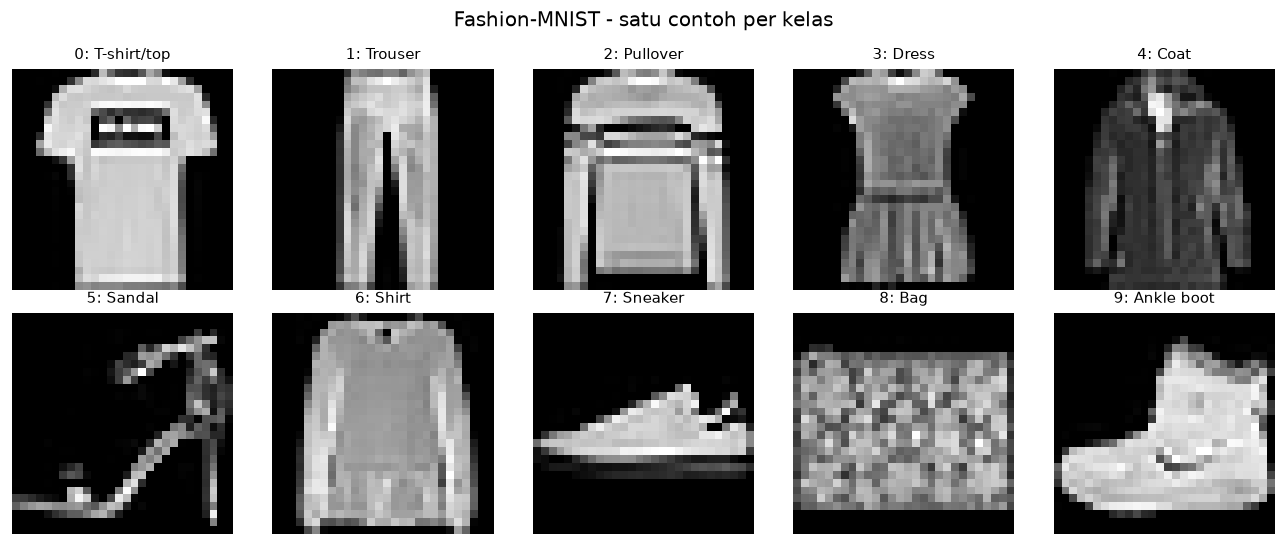
\includegraphics[width=0.92\textwidth]{dataset_samples.png}
\caption{Satu contoh citra asli untuk setiap kelas Fashion-MNIST}
\label{fig:samples-dataset}
\end{figure}

\begin{figure}[H]
\centering
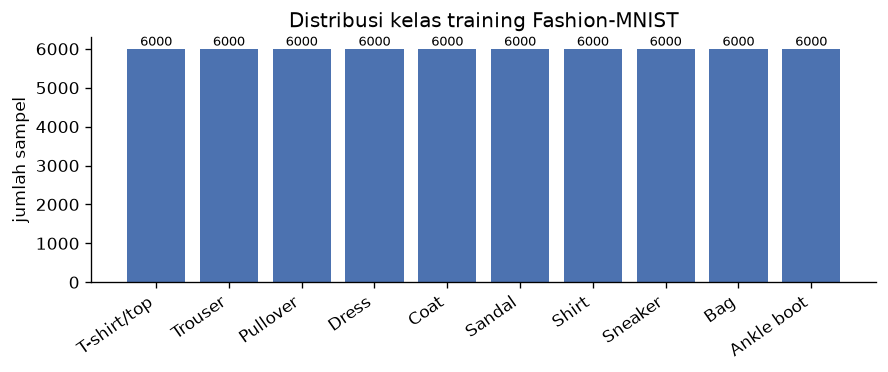
\includegraphics[width=0.85\textwidth]{class_distribution.png}
\caption{Distribusi jumlah sampel per kelas pada data latih}
\label{fig:distribusi}
\end{figure}

\section{Hasil Pelatihan}

Pelatihan 50 epoch selesai dalam 1.061,2 detik (\textit{wall-clock}) pada CPU tanpa percepatan perangkat keras khusus. Rata-rata loss pada beberapa epoch ditunjukkan pada Tabel \ref{tab:loss}. Nilai diambil dari epoch awal, tengah, dan akhir pelatihan.

\begin{table}[H]
\centering
\caption{Ringkasan loss pelatihan pada beberapa epoch}
\label{tab:loss}
\begin{tabular}{|L{1.5cm}|L{4.4cm}|L{4.4cm}|}
\hline
\textbf{Epoch} & \textbf{Loss Discriminator} & \textbf{Loss Generator} \\
\hline
1 & 0,3578 & 3,2119 \\
\hline
3 & 0,4285 & 3,6823 \\
\hline
25 & 1,1315 & 1,2639 \\
\hline
49 & 1,2561 & 0,9481 \\
\hline
50 & 1,2613 & 0,9564 \\
\hline
\end{tabular}
\end{table}

Kurva loss lengkap ditampilkan pada Gambar \ref{fig:loss}. Kedua kurva bergerak saling mendekat dan berosilasi di sekitar nilai 1 pada paruh kedua pelatihan. Pola ini menunjukkan permainan D dan G relatif seimbang, bukan berarti kualitas gambar terus meningkat, karena loss adversarial bersifat relatif terhadap kekuatan lawan.

\begin{figure}[H]
\centering
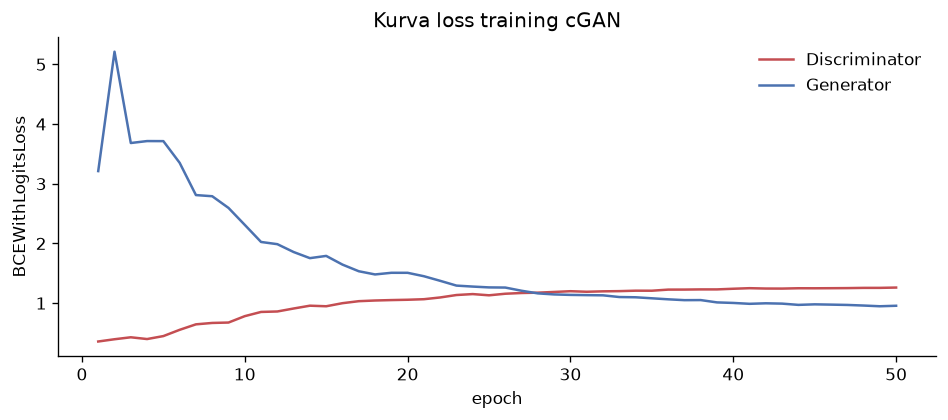
\includegraphics[width=0.88\textwidth]{loss_curve.png}
\caption{Kurva loss Discriminator dan Generator selama 50 epoch}
\label{fig:loss}
\end{figure}

\section{Pengaruh Jumlah Epoch terhadap Kualitas Visual}

Gambar \ref{fig:progresi} membandingkan keluaran tiga checkpoint berbeda menggunakan noise dan label yang sama. Perbandingan ini memberi gambaran langsung mengenai perkembangan bentuk, terlepas dari nilai loss. Pada epoch awal, citra masih berupa gumpalan abu-abu tanpa siluet yang jelas. Pada epoch pertengahan, bentuk kaus, tas, dan sepatu mulai muncul. Pada epoch akhir, kontras dan struktur siluet lebih tegas, meskipun masih terdapat kekaburan dan derau di latar.

\begin{figure}[H]
\centering
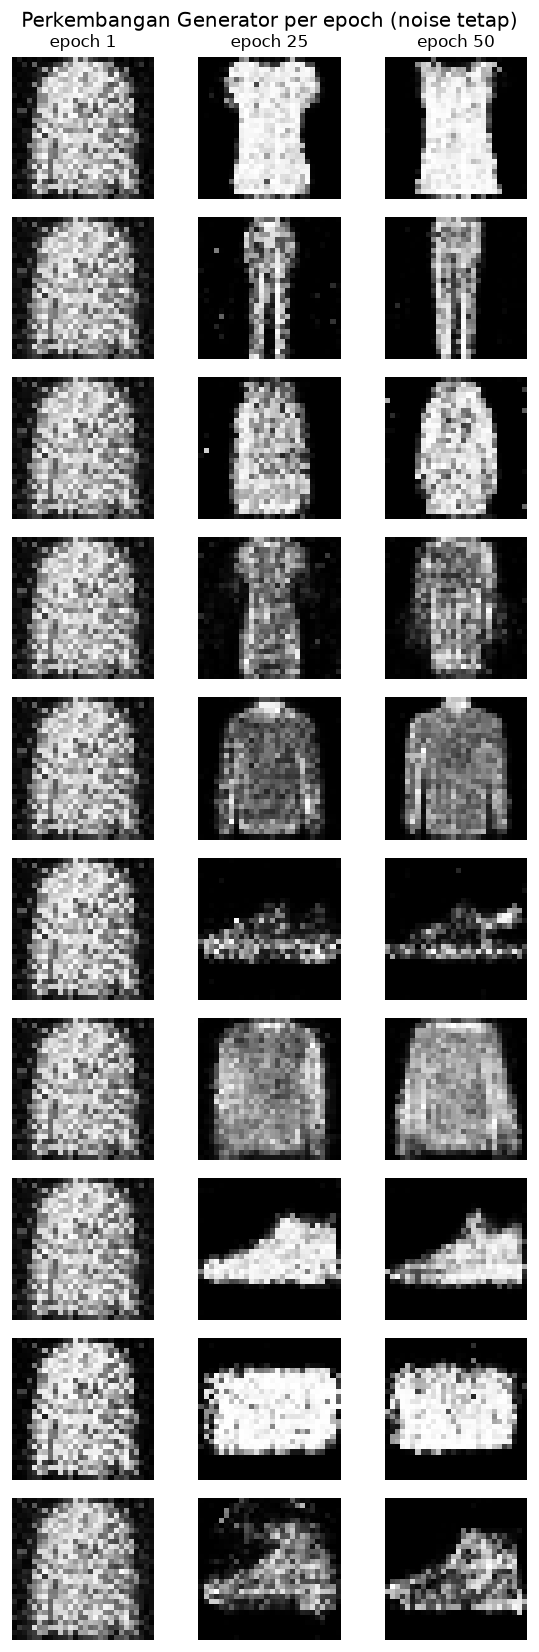
\includegraphics[height=0.82\textheight]{progression_by_epoch.png}
\caption{Perkembangan keluaran Generator pada epoch 1, 25, dan 50 dengan noise tetap}
\label{fig:progresi}
\end{figure}

\section{Sampel Hasil Generator}

Gambar \ref{fig:sampel-kelas} menyajikan empat sampel berbeda untuk setiap kelas dari checkpoint terakhir. Bentuk yang khas paling jelas terlihat pada kelas \textit{Trouser}, \textit{Bag}, \textit{Sneaker}, dan \textit{Ankle boot}. Sebaliknya, \textit{Shirt}, \textit{Pullover}, \textit{Coat}, dan \textit{Dress} cenderung saling menyerupai karena siluetnya beririsan.

\begin{figure}[H]
\centering
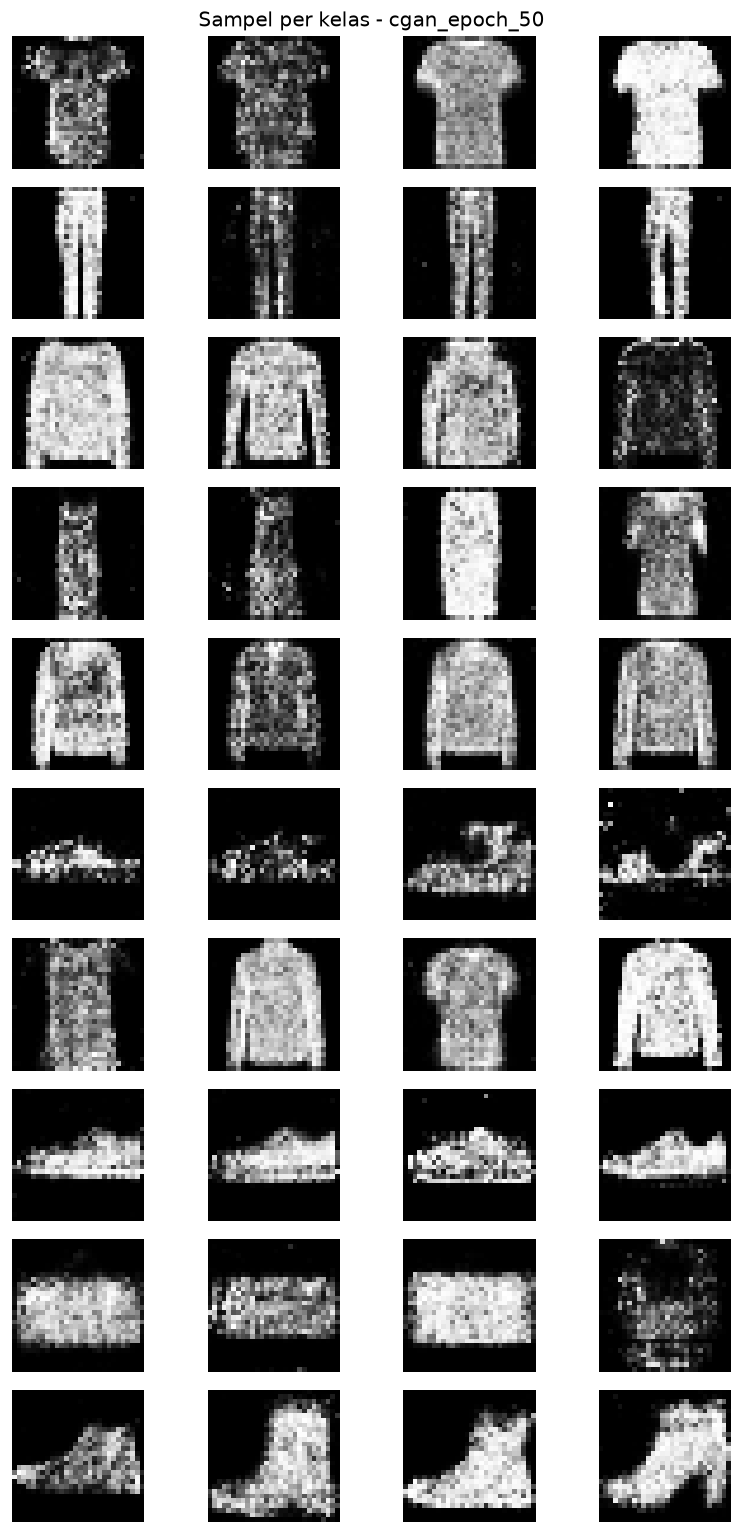
\includegraphics[height=0.86\textheight]{samples_per_class.png}
\caption{Empat sampel hasil Generator untuk setiap kelas pada epoch 50}
\label{fig:sampel-kelas}
\end{figure}

Grid satu gambar per kelas ditunjukkan pada Gambar \ref{fig:grid}. Bentuk grid ini dipakai untuk memeriksa secara cepat apakah \textit{conditioning} label bekerja, karena setiap kolom mewakili label berbeda dari satu vektor noise yang sama.

\begin{figure}[H]
\centering
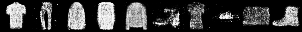
\includegraphics[width=0.62\textwidth]{grid_one_per_class.png}
\caption{Grid satu sampel per kelas dari noise yang sama}
\label{fig:grid}
\end{figure}

\section{Keragaman Sampel}

Selain kesesuaian kelas, diperlukan pemeriksaan terhadap \textit{mode collapse}, yaitu kondisi ketika Generator menghasilkan variasi yang hampir sama untuk semua noise. Gambar \ref{fig:keragaman} menampilkan dua belas sampel per kelas untuk empat kelas representatif. Variasi bentuk masih terlihat, misalnya perbedaan kemiringan lengan pada kelas \textit{T-shirt} serta variasi sol pada \textit{Sneaker}. Dengan demikian, \textit{mode collapse} total tidak terjadi, meski variasi bentuknya tidak selebar data asli.

\begin{figure}[H]
\centering
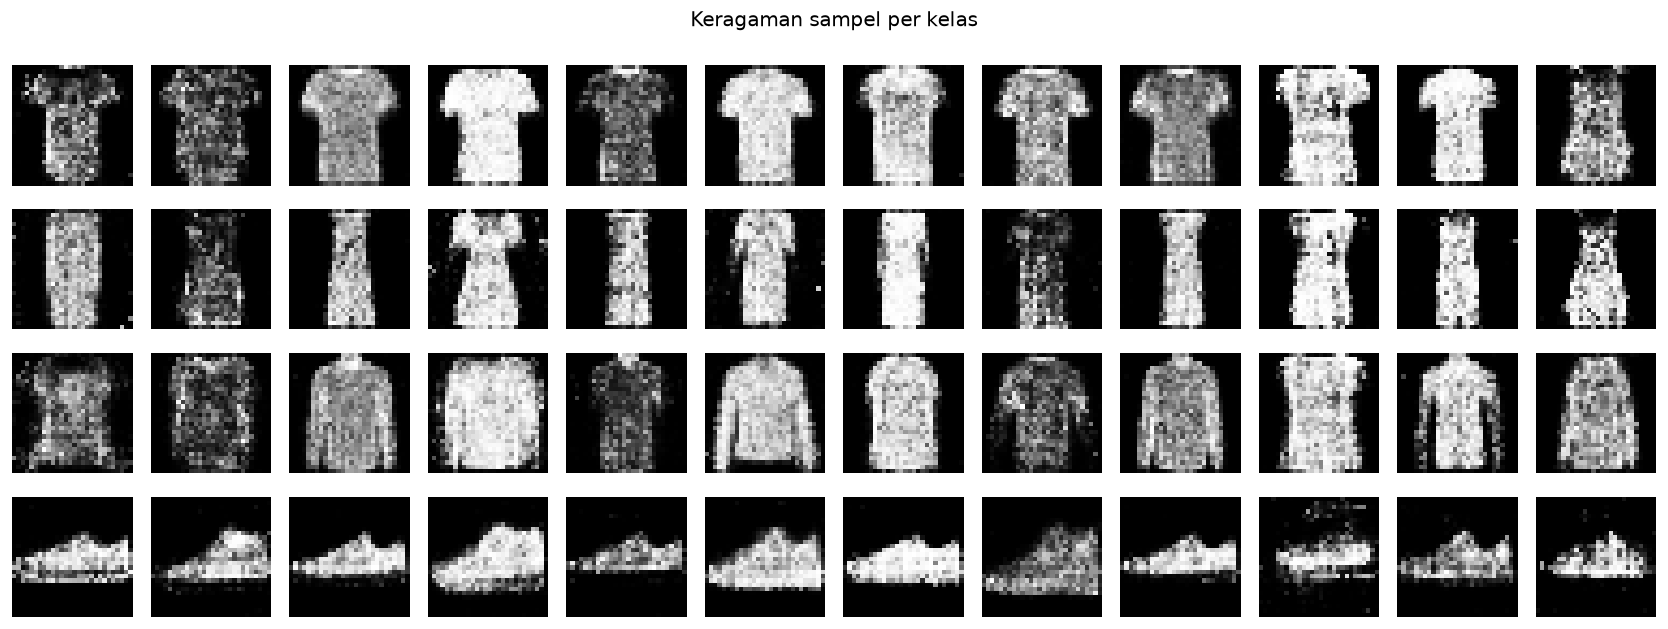
\includegraphics[width=\textwidth]{diversity_per_class.png}
\caption{Keragaman sampel dalam kelas yang sama (dua belas sampel)}
\label{fig:keragaman}
\end{figure}

\section{Hasil Evaluasi Kuantitatif}

Classifier MLP dilatih lima epoch pada data asli dan mencapai akurasi 0,8755 pada 10.000 citra uji. Angka ini menjadi pembanding untuk gambar generator. Hasil pada 100 gambar per kelas dirangkum pada Tabel \ref{tab:akurasi}.

\begin{table}[H]
\centering
\caption{Akurasi classifier pada gambar generator per kelas (100 sampel per kelas)}
\label{tab:akurasi}
\begin{tabular}{|L{1.1cm}|L{2.6cm}|L{1.9cm}|L{3.3cm}|}
\hline
\textbf{Label} & \textbf{Kelas} & \textbf{Akurasi} & \textbf{Keterangan} \\
\hline
0 & \textit{T-shirt/top} & 0,94 & tinggi \\
\hline
1 & \textit{Trouser} & 1,00 & tertinggi \\
\hline
2 & \textit{Pullover} & 0,84 & sedang \\
\hline
3 & \textit{Dress} & 0,89 & sedang \\
\hline
4 & \textit{Coat} & 0,75 & rendah \\
\hline
5 & \textit{Sandal} & 0,99 & tinggi \\
\hline
6 & \textit{Shirt} & 0,62 & terendah \\
\hline
7 & \textit{Sneaker} & 0,88 & sedang \\
\hline
8 & \textit{Bag} & 0,93 & tinggi \\
\hline
9 & \textit{Ankle boot} & 0,83 & sedang \\
\hline
\multicolumn{4}{|l|}{\textbf{Rata-rata} generator 0,8670 (asli 0,8755)} \\
\hline
\end{tabular}
\end{table}

Gambar \ref{fig:akurasi} memvisualkan perbandingan yang sama dalam bentuk diagram batang. Rata-rata akurasi generator 0,8670 hanya berselisih 0,0085 dari akurasi data asli. Selisih kecil ini perlu ditafsirkan hati-hati. Karena semua kelas pakaian berjumlah seimbang dan classifier cukup akurat, hasil ini menunjukkan bahwa mayoritas gambar generator sudah menyerupai kelas asalnya menurut pandangan classifier. Namun, classifier yang dipakai berkapasitas kecil sehingga belum tentu menangkap detail tekstur dan cacat lokal yang terlihat oleh mata manusia.

\begin{figure}[H]
\centering
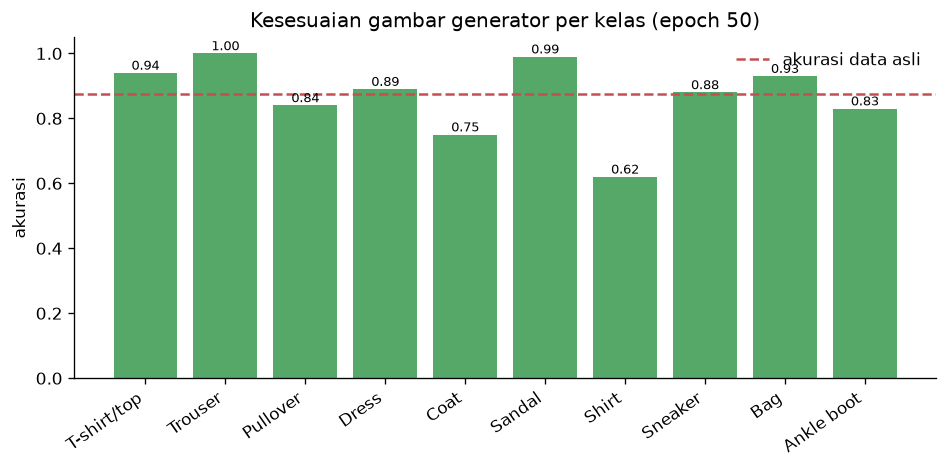
\includegraphics[width=0.88\textwidth]{classifier_accuracy.png}
\caption{Akurasi kesesuaian kelas gambar generator dengan garis pembanding akurasi data asli}
\label{fig:akurasi}
\end{figure}

\section{Pembahasan}

Tiga temuan utama dapat disimpulkan dari hasil di atas. Pertama, \textit{conditioning} label terbukti berpengaruh: gambar dengan label berbeda memiliki distribusi bentuk yang khas, dan kelas dengan siluet unik memperoleh akurasi tertinggi. Kedua, kelas yang secara visual mirip memperoleh akurasi terendah, yang konsisten dengan keterbatasan MLP dalam menangkap perbedaan halus seperti kerah dan panjang lengan. Ketiga, loss adversarial tidak sejalan lurus dengan kualitas visual; pada paruh kedua pelatihan, loss D justru naik sementara bentuk gambar membaik.

Perbandingan dengan arsitektur konvolusional menunjukkan bahwa DCGAN menghasilkan detail yang lebih tajam karena memanfaatkan struktur spasial \citep{radford2015dcgan}. Batasan ini sesuai dengan pilihan metodologis pada Bab III, dan perbaikan berupa lapisan konvolusi dapat diperlakukan sebagai eksperimen lanjutan terpisah tanpa mengubah kontrak data yang sudah ada.

Dari sisi rekayasa perangkat lunak, pemisahan modul menghasilkan pengujian yang dapat dijalankan cepat. Seluruh 36 pengujian lulus pada CPU dalam hitungan detik, termasuk pengujian bahwa perubahan label benar-benar memengaruhi keluaran Generator saat bobot dikendalikan, serta pengujian bahwa resume dari checkpoint melanjutkan penomoran epoch dengan benar.

\chapter{Kesimpulan}

\section{Kesimpulan}

Berdasarkan hasil implementasi dan eksperimen, dapat disimpulkan hal berikut.
\begin{enumerate}
    \item Conditional GAN berbasis MLP berhasil diimplementasikan dari komponen dasar PyTorch dan mampu membangkitkan citra Fashion-MNIST $28\times28$ pada sepuluh kelas. Label \textit{one-hot} yang digabungkan dengan noise pada Generator serta dengan piksel pada Discriminator terbukti memengaruhi keluaran, baik melalui pengujian unit terkontrol maupun melalui perbedaan bentuk antarkelas pada hasil visual.
    \item Pipeline data, training, pembangkitan, dan evaluasi berjalan dengan konfigurasi tercatat dan seed tetap. Pelatihan 50 epoch pada CPU selesai dalam 1.061,2 detik dengan loss akhir Discriminator 1,2613 dan Generator 0,9564. Seluruh 36 pengujian unit lulus.
    \item Rata-rata kesesuaian kelas gambar generator mencapai 0,8670 dengan pembanding akurasi classifier pada data asli 0,8755. Kelas bersiluet khas memperoleh akurasi tinggi (\textit{Trouser} 1,00; \textit{Sandal} 0,99), sedangkan kelas yang mirip secara visual memperoleh akurasi rendah (\textit{Shirt} 0,62; \textit{Coat} 0,75).
\end{enumerate}

\section{Keterbatasan}

Arsitektur MLP tidak memanfaatkan struktur spasial sehingga detail tepi dan tekstur pakaian masih kabur. Classifier evaluasi berkapasitas kecil dan dilatih singkat, sehingga angka akurasi bersifat relatif dan tidak mengukur kualitas estetika. Metrik yang dipakai tidak memperhitungkan keragaman secara kuantitatif; pemeriksaan \textit{mode collapse} hanya dilakukan secara visual.

\section{Saran Pengembangan}

Pengembangan yang disarankan adalah mengganti atau menambah lapisan konvolusi (misalnya DCGAN) sebagai eksperimen terpisah, menambah metrik keragaman yang tetap tanpa model \textit{pretrained}, serta memperbesar kapasitas classifier evaluasi agar penilaian lebih sensitif terhadap cacat lokal.


\cleardoublepage
\addcontentsline{toc}{chapter}{Daftar Pustaka}
\bibliographystyle{plain}
\bibliography{References}
\cleardoublepage
\addcontentsline{toc}{chapter}{Lampiran}
\chapter*{Lampiran}
\addcontentsline{toc}{section}{A. Struktur Repositori}

Struktur repositori yang dipakai selama pengerjaan ditunjukkan pada Tabel \ref{tab:struktur}. Berkas data, checkpoint, dan hasil eksperimen tidak dimasukkan ke dalam repositori karena ditangani melalui \texttt{.gitignore}.

\begin{table}[H]
\centering
\caption{Struktur direktori repositori}
\label{tab:struktur}
\begin{tabular}{|L{3.9cm}|L{7.1cm}|}
\hline
\textbf{Path} & \textbf{Keterangan} \\
\hline
\texttt{src/fashion\_cgan/models.py} & Generator dan Discriminator MLP beserta validasi masukan \\
\hline
\texttt{src/fashion\_cgan/data.py} & Loader Fashion-MNIST dengan normalisasi $[-1,1]$ dan seed \\
\hline
\texttt{src/fashion\_cgan/train.py} & Prosedur pelatihan, checkpoint, metrik, opsi resume \\
\hline
\texttt{src/fashion\_cgan/generate.py} & Pembangkitan grid citra dari checkpoint \\
\hline
\texttt{src/fashion\_cgan/evaluate.py} & Classifier evaluasi dan pengukuran akurasi per kelas \\
\hline
\texttt{src/fashion\_cgan/utils.py} & Fungsi bantu denormalisasi, metrik, dan penyimpanan grid \\
\hline
\texttt{configs/default.yaml} & Konfigurasi eksperimen \\
\hline
\texttt{tests/} & Pengujian unit model, data, training, generate, evaluasi \\
\hline
\texttt{notebooks/} & Notebook visualisasi laporan dan bahan presentasi \\
\hline
\texttt{docs/} & Arsitektur, rencana implementasi, evaluasi, log sesi AI \\
\hline
\texttt{evidence/} & Bukti sesi pengerjaan tiap anggota \\
\hline
\end{tabular}
\end{table}

\addcontentsline{toc}{section}{B. Perintah Reproduksi}

Seluruh tahapan dapat dijalankan ulang dengan perintah pada Tabel \ref{tab:perintah}. Diasumsikan lingkungan virtual pada direktori \texttt{.venv} sudah terpasang melalui \texttt{pip install -r requirements.txt}.

\begin{table}[H]
\centering
\caption{Perintah reproduksi eksperimen}
\label{tab:perintah}
\begin{tabular}{|L{3.4cm}|L{7.9cm}|}
\hline
\textbf{Tahap} & \textbf{Perintah} \\
\hline
Pengujian & \texttt{python -m pytest tests -q} \\
\hline
Training & \texttt{python -m fashion\_cgan.train --device cpu} \\
\hline
Resume & \texttt{python -m fashion\_cgan.train --resume outputs/cgan\_epoch\_N.pt} \\
\hline
Pembangkitan & \texttt{python -m fashion\_cgan.generate outputs/cgan\_epoch\_50.pt} \\
\hline
Evaluasi & \texttt{python -m fashion\_cgan.evaluate outputs/cgan\_epoch\_50.pt} \\
\hline
Visualisasi & Eksekusi \texttt{notebooks/report\_visuals.ipynb} dari root repositori \\
\hline
\end{tabular}
\end{table}

Pada Windows PowerShell, variabel \texttt{PYTHONPATH} perlu diisi dengan nilai \texttt{src} agar paket \texttt{fashion\_cgan} dapat diimpor.

\addcontentsline{toc}{section}{C. Bukti Sesi Pengerjaan}

Bukti pemakaian asisten AI disimpan terpisah per anggota pada direktori \texttt{evidence/}. Ringkasannya disajikan pada Tabel \ref{tab:evidence}.

\begin{table}[H]
\centering
\caption{Ringkasan berkas bukti per anggota}
\label{tab:evidence}
\begin{tabular}{|L{3.9cm}|L{7.1cm}|}
\hline
\textbf{Anggota} & \textbf{Berkas bukti} \\
\hline
Ivander Dzaky Khairullah & \texttt{session-001-planning.md}, \texttt{session-002-generator-discriminator.md}, \texttt{session-004-preprocessing-training.md} beserta ekspor JSON asli \\
\hline
Muhammad Ragil & \texttt{session-001-data-training-and-github-workflow.md} \\
\hline
Silmi Sila Nia Uma & \texttt{session-001-evaluation.md} \\
\hline
\end{tabular}
\end{table}

\end{document}
